\documentclass{article}
\usepackage[landscape]{geometry}
\usepackage[american]{babel}
\usepackage{merriweather}
\pagestyle{empty}
\usepackage{graphicx}
\usepackage{makecell}
\usepackage{xcolor}
  \definecolor{darkred}{HTML}{6A041D}
  \definecolor{darkgreen}{HTML}{386150}
  \definecolor{darkblue}{HTML}{27213C}
\usepackage{microtype}
\usepackage{multicol}
\usepackage{hyperref}
  \hypersetup{colorlinks=true,allcolors=blue!40!black}
\begin{document}
\def\zoldversion{0.2.4}

\pagecolor{white}
\newcommand\slide[1]{%
  \pagebreak\topskip0pt\vspace*{\fill}%
  \begin{center}\Huge%
  #1
  \end{center}%
  \vspace*{\fill}%
}

\slide{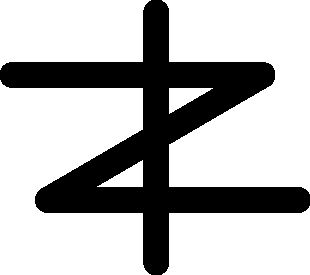
\includegraphics[scale=1]{../images/zerocracy-logo.pdf}\\
Zerocracy, Inc.\\[1em]
\large
Freelance Deck\\
\href{https://www.zerocracy.com}{www.zerocracy.com}}

\slide{
  Gallup \href{https://www.cnbc.com/2018/05/30/70-percent-of-people-globally-work-remotely-at-least-once-a-week-iwg-study.html}{recently found out}
  that the number of American employees
  working remotely rose to 43 percent in 2016 from 39 percent in 2012.
  However, as \href{https://www.entrepreneur.com/article/280749}{noted}
  by Rustam Singh in Entrepreneur,
  ``freelancers are exactly second in line (right after interns),
  to be regarded as the most under-appreciated working population
  on the planet currently.''
}

\slide{
  \newcommand\topic[2]{\vbox{\normalsize\colorbox{darkred}{\color{white}{#1}}\newline\footnotesize#2\vspace{4pt}}}
  What Are The Key Freelance Pitfalls?
  \begin{multicols}{3}
  \raggedright

  \topic{Lack of Control}{
    Qubit Labs, a Ukrainian outsourcer, in their blog post of disappointed
    \href{https://qubit-labs.com/reasons-why-we-will-never-hire-freelancers-again/}{explains}:
    ``You do not know exactly how freelancer works. No matter how
    much you convince yourself, you have no power over freelancers.
    They can deliver the project on time, or not.''}

  \topic{Low Quality}{
    It is often assumed that programmers working remotely without
    close daily supervision produce lower quality of their code
    than their full-time colleagues.}

  \topic{Communication Issues}{
    Reddit and Yahoo \href{http://www.gallup.com/poll/184649/telecommuting-work-climbs.aspx}{banned}
    remote work and Reddit CEO
    \href{https://www.quora.com/Is-Reddit-closing-their-NYC-and-Salt-Lake-City-offices-They-have-asked-all-remote-workers-to-decide-by-the-end-of-2014-if-they-want-to-move-to-San-Francisco-or-leave-the-company}{said}
    that
    ``there were too many times when we just needed to be able
    to walk over and tap someone on the shoulder and discuss
    a complex issue in-depth, right away,'' which is difficult
    to do with remotely distributed freelancers.}

  \topic{Fake Portfolios}{
    Relja Damnjanovic from \href{https://www.toptal.com}{Toptal} describes his personal experience of
    being a victim of identity theft and
    \href{https://www.toptal.com/freelance/freelancer-identity-theft}{says} that,
    ``Unethical people create profiles on open freelance networks,
    pretending to be someone with much more experience and expertise
    than themselves. They use the stolen profile to poach
    jobs, and set higher prices than they're worth.''}

  \topic{IPR Issues}{
    While full-time employees are binded by multi-page NDAs and contracts,
    freelancers, even when they ``work for hire'' are less responsible legally;
    moreover, they are mostly overseas.}

  \topic{High Turnover}{
    As Riia O'Donnell from RecruiterBox
    \href{https://recruiterbox.com/blog/freelance-vs-fulltime-pros-cons-hiring-independent-contractor}{says},
    ``They may be great when they're accessible,
    but be prepared with a Plan B if they're not.''}

  \topic{Absence of Talents}{
    As \href{https://en.wikipedia.org/wiki/Yishan_Wong}{Yishan Wong},
    former CEO of Reddit, \href{https://www.quora.com/How-does-a-business-person-outsource-a-good-developer-programmer-engineer-on-eLance-or-oDesk-I-dont-understand-nor-can-I-differentiate-all-the-latest-programming-languages-What-skill-sets-should-I-be-looking-for/answer/Yishan-Wong}{described}
    his freelance experience, ``it was extremely difficult to find decent engineers who could
    do the things he needed, deliver reliably, and iterate according
    to ongoing testing/customer feedback.''}

  \topic{Lack of Commitment}{
    ``If client site is down, a client can't call a freelancer
    to work on it right at this moment but it's different for an employee,''
    \href{https://imtips.co/disadvantages-hiring-freelancer.html}{says} Shabbir Bhimani,
    a software blogger.}

  \topic{No Accountability}{
    ``A lot of freelancers have no drive and determination, it is
    self-motivated job and if they are having a bad day then it
    is so easy to see why they may not produce high standard work,''
    \href{https://creativebeacon.com/freelancers-bad-reputation/}{says} Creative Beacon.}

  \topic{Good Ones Are Expensive}{
    Even though the \href{https://vulcanpost.com/634361/freelancer-singapore-paypal-survey/}{recent study}
    of PayPal revealed that over 50\% of freelancers are not being paid regularly,
    in order to hire a decent engineer one has to pay double, since,
    as Jay Soriano \href{http://launchastartup.com/odesk-vs-elance/}{explained},
    ``the good freelancers become insulted with the low pricing, and
    the `good enough' freelancers stay but don't feel that they
    have to provide quality because the price is so low.''}

  \topic{Cultural Differences}{
    Anne Loehr claims in her
    \href{https://www.anneloehr.com/2014/11/03/4-steps-maintain-organizational-culture-freelance-employees/}{blog post} that
    ``freelance employees don't fit in with the organizational culture'' and it's a ``management challenge.''}

  \topic{Moody Attitude}{
    As Sara Horowitz, founder of \href{https://www.freelancersunion.org/}{Freelancers Union},
    once \href{http://www.villagevoice.com/2013-02-13/news/a-decade-on-freelancers-union-founder-sara-horowitz-takes-her-fight-mainstream/}{said}:
    ``You work with freelancers and you learn about depression.''
    Anya Kamenetz \href{https://www.fastcompany.com/3006208/why-freelancers-are-so-depressed}{elaborated}
    further in FastCompany, and confirmed that self-employed are indeed
    ``least likely to report themselves as thriving.''}

  \topic{Mixed Priorities}{
    According to \href{https://www.daxx.com/article/problems-bad-freelancers}{DAXX},
    an outsourcer headquartered in The Netherlands, you should
    ``be prepared to missed deadlines due to weddings, birthdays, funerals, relatives
    getting sick unexpectedly, and all kinds of similar excuses.''}
\end{multicols}}

\slide{Zerocracy has invented how to mitigate all these pitfalls and painlessly work with freelancers.}

\slide{
  \newcommand\topic[2]{\vbox{{\normalsize\colorbox{darkgreen}{\color{white}{#1}}}\newline\footnotesize#2\vspace{6pt}}}
  How Zerocracy Does That?
  \begin{multicols}{3}
  \raggedright

  \topic{Pay By Result}{
    Unlike Upwork and similar systems,
    our freelancers are being paid only for the results they deliver,
    not the time they spend in the office or remotely.}

  \topic{Microtasking}{
    The \href{https://www.xdsd.org}{XDSD} methodology we \href{https://www.xdsd.org/XDSD-WhitePaper.pdf}{invented}
    encourages programmers to break down their scope of work
    into \href{https://www.yegor256.com/2017/11/28/microtasking.html}{small increments}
    and make sure they are delivered only when the quality
    is acceptable.}

  \topic{Communication Discipline}{
    All project communications happen inside ticket tracking systems, like
    Jira, Trello, or GitHub; no informal
    \href{https://www.yegor256.com/2014/10/07/stop-chatting-start-coding.html}{chats of meetings}
    are allowed.}

  \topic{Senior Developers Only}{
    There are only highly-skilled and professional developers in the platform,
    because everybody else simply can't survive under the pressure of our
    quality expectations.}

  \topic{Rating System}{
    Each activity completed or failed by a programmer has certain consequences
    in reputation points, which are accumulated in programmer's profile and
    affect their pay rates.}

  \topic{High Rates}{
    We pay over the market, in order to be able to demand the highest
    quality; e.g., a Java programmer from Poland may earn \$60-80 per hour
    (pro-rated by the results delivered).}

  \topic{Strict Policy}{
    The management methodology is explained in the
    \href{https://www.zerocracy.com/policy}{Policy} document (over 50 paragraphs), which
    explicitly regulates everything freelancers are doing in a project.}

  \topic{Zerocrat Chatbot}{
    The project management role is played by a \href{https://www.yegor256.com/2018/03/21/zerocracy-announcement.html}{chatbot},
    which
    ``talks'' to programmers via Telegram, Slack, and GitHub, gives them
    instructions and collects their results.}

  \topic{Mentorship}{
    Each new freelancer in the platform has to have a mentor among those
    who already know how the system works, which ensures easily
    adopting of new members to our community and our quality expectations.}

  \topic{Sandbox}{
    All newcomers are being tested in so called ``sandbox'' projects, which
    are sponsored by Zerocracy, where freelancers while being fully paid,
    experiment with the management model and get ready for real projects.}

  \topic{Double Peer Reviews}{
    Each software code increment, also known as pull request, has to be
    reviewed by at least two other programmers, which makes sure the quality
    is not compromised easliy.}

  \topic{Quality Assurance}{
    A mandatory quality assurance role in each project validates that all
    rules of work are enforced and the quality is not compromised.}
\end{multicols}}

\slide{An effective utilization of a growing army of freelancers,
  which only Zerocracy is capable of doing at the moment,
  will greately benefit almost any smart software company.}

\slide{
  \newcommand\topic[2]{\vbox{{\normalsize\colorbox{darkblue}{\color{white}{#1}}}\newline\footnotesize#2\vspace{6pt}}}
  Where Do We Find Freelancers?
  \begin{multicols}{3}
  \raggedright

  \topic{Conferences}{
    We regularly speak at \href{https://www.yegor256.com/talks.html}{software conferences} and present our novel
    ideas about management; thanks to the attractiveness of the concept
    we are getting a few ``join'' requests per day from freelancers.
    We are planning to attend more conferences in the future and organize our own, about freelance and management.}

  \topic{Blogs}{
    We write about our system and its management principles in
    \href{https://www.zerocracy.com/blog.html}{our blog} and in the
    \href{https://www.yegor256.com}{blog} of our CEO.
    We are planning to motivate our programmers and customers to write more actively for our blog.}

  \topic{YouTube Videos}{
    We promote the concept via our \href{https://www.youtube.com/channel/UCxZAzmY_OPw40I1-YStWqhw}{YouTube channel}
    and the \href{https://www.youtube.com/c/yegor256?sub_confirmation=1}{channel} of our CEO.
    We are planning to do more interactive webinars and online interviews.}

  \topic{Open Source}{
    Our entire software platform is \href{https://github.com/zerocracy}{open source},
    all our sandbox projects are open source. Moreover, our CEO organizes a regular
    annual Quality Award for open source developers. This is how we attract a large
    community of the most active programmers and share our ideas with them.
    We are planning to sponsor more open source initiatives in the future.}

  \topic{Books}{
    \href{https://www.yegor256.com/}{Yegor Bugayenko}, our CEO, is a famous tech writer, an author
    of \href{https://www.yegor256.com/elegant-objects.html}{\textit{Elegant Objects}},
    a book series on object-oriented programming, and
    a rather famous tech \href{https://www.yegor256.com}{blogger}.
    His most recent book \href{https://www.yegor256.com/code-ahead.html}{\textit{Code Ahead}}
    promotes the ideas of freelancing and our platform.
    We are planning to publish more books about our concepts and our solution.}

  \topic{Telegram Chat}{
    We have a dedicated Telegram \href{https://t.me/zerocracy}{chat} for our
    early adopters, followers, freelancers, and even customers. In the chat
    we discuss how the platform works, resolves issues, and provide help
    to newcomers.}
\end{multicols}}

\slide{The future of software development will certainly depend on freelancers working remotely.
  The question is who will able to find a way to manage them effectively.
  Zerocracy has done it already.}

\slide{%
  \Large 555 Bryant Str, Ste 470\\
  \Large Palo Alto, CA 94301\\
  \Large 408.692.4742\\
  \Large \href{mailto:team@zerocracy.com}{team@zerocracy.com}\\[1em]
  \normalsize\texttt{\zoldversion\qquad\today}}

\end{document}
